%
% File acl2018.tex
%
%% Based on the style files for ACL-2017, with some changes, which were, in turn,
%% Based on the style files for ACL-2015, with some improvements
%%  taken from the NAACL-2016 style
%% Based on the style files for ACL-2014, which were, in turn,
%% based on ACL-2013, ACL-2012, ACL-2011, ACL-2010, ACL-IJCNLP-2009,
%% EACL-2009, IJCNLP-2008...
%% Based on the style files for EACL 2006 by 
%%e.agirre@ehu.es or Sergi.Balari@uab.es
%% and that of ACL 08 by Joakim Nivre and Noah Smith

\documentclass[11pt,a4paper]{article}
\usepackage[hyperref]{acl2018}
\usepackage{times}
\usepackage{latexsym}
\usepackage{graphicx}
\graphicspath{ {images/} }
\usepackage{amsmath,amsfonts,amssymb}
\usepackage{bbm}
\usepackage{url}
\usepackage{multirow}

\DeclareMathOperator*{\argmin}{arg\,min}

% \aclfinalcopy % Uncomment this line for the final submission
 \def\aclpaperid{13} %  Enter the acl Paper ID here

%\setlength\titlebox{5cm}
% You can expand the titlebox if you need extra space
% to show all the authors. Please do not make the titlebox
% smaller than 5cm (the original size); we will check this
% in the camera-ready version and ask you to change it back.

\newcommand\BibTeX{B{\sc ib}\TeX}

\title{\textit{BioAMA}: Towards an End to End BioMedical Question Answering System}

\author{Vasu Sharma*, Nitish Kulkarni*, Srividya Pranavi Potharaju*, \\\textbf{Gabriel Bayomi*, Eric Nyberg, Teruko Mitamura}\\
  Language Technologies Institute \\
  School Of Computer Science \\
  Carnegie Mellon University \\
  {\tt [vasus, nitishkk, spothara, gbk, ehn, teruko] @cs.cmu.edu}\\
  }


    
\date{}

\begin{document}
\maketitle
\begin{abstract}
This paper describes our Biomedical Question Answering model, \textit{BioAMA} on task 5b of the fifth edition of the annual BioASQ challenge \cite{bioasq}. In this work we focus on a wide variety of question types including  factoid, list based and yes/no type questions and generate both exact and well formed `ideal' answers for each of these question types. We combine effective information retrieval based techniques for retrieving most relevant snippets with respect to a question with statistical ranking and sentence extraction based methods to obtain an end to end complete system which achieves the state of the art on ideal answer type questions yielding a ROGUE-2 score of  0.72 and a ROUGUE-SU4 score of 0.71 which is a 7\%  improvement over the previous best model.\\We also propose a novel approach for tackling the yes/no, factoid and list type questions and obtain competitive results on the BioASQ dataset.

\end{abstract}



\section{Introduction}
In the era of ever advancing medical sciences and the age of the internet, a remarkable amount of medical literature is constantly being posted online. This has led to a need for an effective retrieval and indexing system which can allow us to extract meaningful information from these vast knowledge sources. One of the most effective and natural ways to leverage this huge amount of data in real life is to build a Question Answering system which will allow us to directly query this data and extract meaningful and structured information in a human readable form. In this paper, we present our system ``\textit{BioAMA}: Biological Ask Me Anything" which is an end-to-end biomedical question answering system capable of handling a very large variety of questions types on the BioASQ dataset.  \\
The key novel contributions we make are as follows:
\begin{enumerate}
    \item \textbf{State of the art model on ideal answer type questions}: Our proposed \textit{BioAMA} system attains the state of the art results on the ideal answer type questions on the Task 5b of the BioASQ dataset yielding a 7\%  improvement over the previous state of the art system from \cite{khyati-paper}.
    \item \textbf{Novel framework for Yes/No type QA}: 
    We introduce a novel NLI-based approach for answering the Yes/No style questions in the BioASQ dataset. We model these questions as a Textual Entailment (TE) problem and use Hierarchical Convolutional Neural Network based Infersent models \cite{Infersent} to answer this type of questions. To address the problem of lack of adequate training data, we also introduce a novel embedding projection technique which allows for effective transfer learning from models trained on larger datasets with a different vocabulary to work on the much smaller BioASQ dataset.
    \item \textbf{A novel two-stage approach to answer Factoid and List type questions}: 
    In our \textit{BioAMA} model we introduce a novel 2 step pipeline to deal with the factoid and yes/no type questions. We first use a number of biomedical Named entity extractors to generate a candidate answer set in a totally unsupervised setting and then use a supervised ranking algorithm to generate the final predictions.
    \item \textbf{Improving the Maximum Marginal Relevance (MMR) framework}: We improve upon the MMR framework for relevant sentence selection from the chosen snippets. The use of MMR for sentence selection was introduced in the work of Khyati et al. \shortcite{khyati-paper}. We improve upon this framework by experimenting with a number of more informative similarity metrics than the vanilla Jaccard similarity metric they use.

\end{enumerate}
    %\item \textbf{Incorporating Information retrieval in the Question Answering pipeline}:
    %We incorporate Indri and BM25 based features in our pipeline to allow for effective information retrieval from the biomedical knowledgebase which allows us to choose the snippets which are most relevant to a given question. 
    %\item \textbf{Statistical ranking models}: We use the powerful LeTOR framework to allow for ranking of our snippets chosen by the information retrieval mechanism. This allows us to maximize the information we extract from the snippets which are deemed more relevant to a specific question. This also blends in well with our MMR framework which makes use of the ranking framework to extract the most relevant and non-repetitive information from the chosen snippets.
    
    The rest of the paper is organized as follows. Section \ref{lit} presents the prior work on this problem followed by details of the BioASQ challenge and dataset in Section \ref{Dataset}. We present our approach and results for the ideal answer type questions in Section \ref{approach1} and for the exact answer type generation in Section \ref{approach2}. Finally we present the conclusions and future directions of our work in Section \ref{future}.
\section{Relevant Literature}
\label{lit}
Biomedical Question answering has always been a hot topic of research among the QA community at large due to the relative significance of the problem and the challenge of dealing with a non standard vocabulary and vast knowledge sources. The BioASQ challenge has seen large scale participation from research groups across the world. One of the most prominent among such works is from Khyati et al. \shortcite{khyati-paper} who use  extractive summarization techniques to address this task and experiment with different biomedical ontologies and various algorithms including agglomerative clustering, Maximum Marginal Relevance (MMR) and sentence compression. However they only address the ideal answer generation with their model and don't use the vast amount of information present in the PubMed sources only using the snippets for answering the questions. Peng et al. \shortcite{fudan} in their BioASQ submission use a 3 step pipeline for generating the exact answers for the various question types. The first step is question analysis where they subdivide each question type into finer categories and classify each question into these subcategories using a rule based system. They then perform candidate answer generation using PubTator and Stanford POS tagger. A word frequency based approach is then used to rank the candidate entities. Wiese et al. \shortcite{fastqa} propose a neural QA based approach to answer the factoid and list type questions where they use FastQA: a machine comprehension based model \cite{fastqa-squad} and pretrain it on the SquaD dataset \cite{squad} and then finetune it on the BioASQ dataset. They report state of the art results on the Factoid and List type questions on the BioASQ dataset. Another prominent work is from Sarrouti and Alaoui \shortcite{usmba} who handle the generation of the exact answer type questions. They use a sentiment analysis based approach to answer the yes/no type questions making use of SentiWordNet for the same. For the factoid and list type questions they use UMLS metathesaurus and term frequency metric for extracting the exact
answers. They also use the BM25 model and UMLS concepts for retrieving the ideal answers.

\section{The BioASQ challenge}
\label{Dataset}
BioASQ challenge \cite{bioasq} is a large scale biomedical question answering and semantic indexing challenge which has been running as an annual competition since 2013. %This challenge assesses the ability of systems to semantically index very large numbers of biomedical scientific articles, and to return concise and user-understandable answers to given natural language questions by combining information from biomedical articles and ontologies.
We particularly deal with the Phase B of the challenge which deals with large scale biomedical question answering. The dataset provides a set of questions and snippets from Pubmed which are relevant to the specific question. It also provides users with a question type and urls of the relevant pubmed articles itself. The 5b version of this dataset consists of 1,799 questions.\\
The questions were broken up into 3 distinct question types namely:\\
\begin{enumerate}
    \item \textbf{Factoid type}: This question type has a single entity as the ground truth answer and expects the systems to output a set of  entities ordered in relevance order as answer and the systems are evaluated using Mean reciprocal rank \cite{MRR} of the answer entities with reference to the ground truth answer entity.
    \item \textbf{List type}: This answer type expects the system to return an unordered list of entities as answer and evaluates them using a F score based metric against a list of reference answer entities which can vary in number.
    \item \textbf{Yes/No type}: This question type asks the systems to answer a given question with a binary output namely yes or no. The questions typically require reasoning and inference over the evidence snippets to be able to answer the questions correctly.
\end{enumerate}

The dataset expected the participants to generate 2 types of answers namely exact and ideal answers. 
In ideal answers the systems are expected to generate a well formed paragraph for each of the question types which explains the answer to the question. They call these answers `ideal' because it is what a human would expect as an answer by a peer biomedical scientist. In the exact answers the systems are expected to generate ``yes" or ``no" in the case of yes/no questions, named entities in the case of factoid questions and list of named entities in the case of list questions.



\section{Ideal Answers}
\label{approach1}
This section describes our efforts to address the ideal answer category where the goal is to produce a query-based, relevant, non redundant and coherent summary answer from multiple snippets and documents. 

 \begin{figure*}
     \centering
     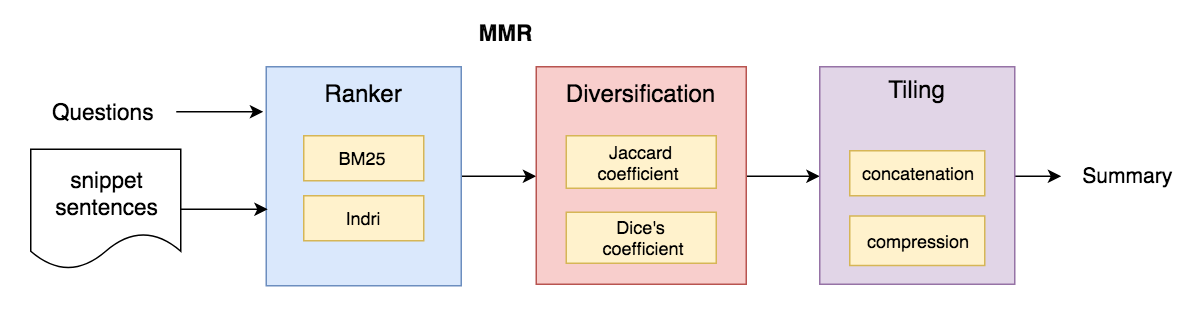
\includegraphics[scale=0.6]{images/pipeline_summary.png}
     \caption{Pipeline for ideal answer generation}
     \label{fig:ideal_answers_pipeline}
 \end{figure*}

Our pipeline for ideal answer comprises three stages. The first stage involves pre-processing of the snippets with creating candidate sentences and ranking the sentences as per various retrieval models described in the following sections. The retrieval model scores form the soft positional component introduced in the MMR algorithm. This brings us to the second stage of the pipeline, sentence selection. We select the top 10 best sentences for generating an ideal answer. The third and final stage involves tiling together the selected sentences to generate a coherent, non redundant, ideal answer for the given question. % as mentioned in
% TODO: Add reference
 We describe our improvements to the pipeline that can be applied to all the above categories with primary focus being summary type questions as described in Section \ref{Dataset}.
The subsequent subsections explain the full pipeline for ideal answer type questions in detail. A brief overview of the pipeline is shown in Figure \ref{fig:ideal_answers_pipeline}.



\subsection{Question-Sentence Retrieval}
In this section, we describe various approaches which we adapted, to improve the initial retrieval of candidate sentences that helped to better formulate the answer.

% \subsubsection{BM25}
% BM25 \cite{BM25} is a standard tf-idf based retrieval algorithm relying on bag of words approach for document retrieval. We considered every question to be independent and built an inverted index over the relevant snippets following the standard methods. Since the snippets are short paragraphs and the question is of moderate length, we tuned BM25 parameters accordingly. We customized the pre-processing by creating our own set of stop words that excluded certain bio-medical entities which might have been considered an English stop-word.
% %\[Score(D, Q) = \sum_1^n IDF(q_i) \frac{f(q_i, D) (k_1 + 1)}{f(q_i, D) + k_1 (1- b + b . \frac{|D|}{avgdl})} \]



\subsubsection{Indri}

Indri \cite{Indri} is a retrieval model based upon statistical language models using query likelihood approach. We assumed a uniform prior over the sentences and ranked the candidate sentences based on the probability of the question given the sentence. We adapted two stage smoothing for estimating the probability values that takes into account both the query (which is question in this context) and sentences characteristics. 

The probability / Indri score for a candidate sentence is estimated in a collection (C) of snippets as follows:
\begin{align}
    & p(q_i|d) = (1-\lambda) p_{mle} (q_i|d) + \lambda p_{mle} (q_i|C) \label{eq1} \\ 
    & p_{mle}(q_i|d) = 
    \frac{tf + \mu  p_{mle}(q_i|C)}{length(d) + C} \label{eq2} \\ 
    & p_{mle}(q_i | C) = \frac{ctf}{length(C)}
\end{align}

In equation \ref{eq1} , $\lambda$ is the coefficient for linear interpolation based smoothing. It is used for question length smoothing. Since the questions are of moderate length, after tuning, the best value of $\lambda$ is attained at 0.75

In equation \ref{eq2} $\mu$ is parameter for Bayesian smoothing using Dirichlet priors. It is used for sentence length normalization. Since sentences of snippets can be of varying lengths, after tuning, the best value of $\mu$ is attained at 5000.

Both of the above smoothing techniques do two different things, the mixture model (interpolation) compensates for differences in the word importance (gives idf-effects) and the Dirichlet prior improves the estimates of the sentence sample which supports our decision to use two stage smoothing. 

% \subsubsection{LeToR}

% Learning to Rank \cite{Letor} is widely used, supervised learning approach for ranking the candidate sentences. We propose a new technique to create gold data for training the LeToR model. For every training data sample, we created a golden ranking of the sentences by ranking the candidate sentences from all the given snippets using golden ideal answer as the question following BM25 algorithm. For feature engineering part of LeToR, we considered different semantic, statistical and language model based features.
% \begin{itemize}
%     \item \textbf{Tf-Idf based}: BM25 score of the sentence
%     \item \textbf{Language model based}: Indri score of the sentence
%     \item \textbf{Semantic}: Count of the Named Entities in each sentence.
%     \item \textbf{Biomedical entities}: We obtained the biomedical entities from biomedical entity extraction tools like PubTator \cite{pubtator}, Lingpipe \cite{lingpipe} and GramCNN \cite{gramcnn}.
% \end{itemize}
% BM25, Indri algorithms were adapted as features for LeToR which was our final model for ranking candidate sentences


\subsection{Sentence Selection}
Once the top most relevant snippets have been chosen, we want to choose sentences from these snippets which are most relevant to a specific question. In this section we demonstrate how this selection is done.

\subsubsection{MMR}

We use Maximum Marginal Relevance(MMR) algorithm \cite{MMR} as our basic foundation algorithm for sentence selection. In contrast to the vanilla Jaccard similarity metric as used in \cite{khyati-paper} for a similar task, we experimented with other similarity metrics which performed consistently better over the former for different test datasets. MMR ensures the selected set contains non redundant yet complete information. The sentences are selected based on two aspects, the sentence's relevance to the question and how different it is to the already selected sentences. At each step we select a document to append to the ranking based on the equation below..
\begin{multline}
     d_i = argmax (\lambda \cdot sim(q, d_i)  \\  - (1 - \lambda) \cdot max(sim_{sent}(d_i, d_j) ) ) \label{eq4}
\end{multline}
   

 We define a custom similarity metric between documents which uses positional values of sentences from the initial ranking as follows:
\begin{multline}
  sim_{sent}(di, dj) = ( 1 - \beta) \cdot (1 - \frac{rank(s_i)}{n}) \\+ \beta \cdot sim(d_i, d_j) 
\end{multline}
Here, $sim_{sent}(di, dj)$ is the sentence to sentence similarity, $sim(q, di)$  is the question - sentence similarity, $rank(s_i)$ is the rank of the snippet which contains the sentence $d_i$, $S$ are Sentences already selected for summary i.e. which are ranked above this position. In the above equation, we tried various metrics to account for the sentence to sentence similarity. In case $\beta$ is 0, equation \ref{eq4} becomes the standard MMR, which we identify with CoreMMR. In all other cases, equation \ref{eq4} is identified as our SoftMMR that also includes the soft scoring based on position of sentences.

\subsubsection{Dice's similarity Coefficient (DSC)}

Dice's similarity Coefficient (DSC) \cite{dice} is a quotient of similarity between two samples and ranges between 0 and 1. It is used to compare similarity of two strings using bigrams. It is different from the Jaccard coefficient which counts intersecting words only once in both the numerator and denominator. It is calculated as follows 
\begin{equation}
    dsc = \frac{2 * n_t}{n_x + n_y}
\end{equation}
where $n_t$ is the number of character bigrams found in both strings, $n_x$ is the number of bigrams in string $x$ and $n_y$ is the number of bigrams in string $y$
\subsection{\textbf{Evaluation}} The pipeline described above is primarily designed to improve the Rouge evaluation metric \cite{Rougue}. This metric might not necessarily reflect the human readability aspect of the answer. MMR, to some extent improves readability by reducing the redundancy in the generated answers.
Results for ideal answers for Task 5 phase b are shown in Table \ref{tab:rouge_extractive_summarization}.

\begin{table}[t!]
    \centering
    \begin{tabular}{|l|c|c|}
         \hline
            Experiment & Rouge-2 & Rouge-SU4 \\
        \hline
        \hline
        baseline & 0.7064 & 0.6962 \\
        \hline
        $\beta$ = 0.5, SoftMMR,  & 0.7175 & 0.7110  \\ 
        BM25, Jaccard&&\\
        \hline
        $\beta$ = 0.5, SoftMMR, & 0.7193 & 0.7106  \\ 
        BM25, Dice&&\\
        \hline
        $\beta$ = 0.0, CoreMMR & 0.7065 & 0.6998  \\ 
        BM25, Dice&&\\
        \hline
        $\beta$ = 0.6, SoftMMR & 0.7133 & 0.7053  \\ 
        BM25, Dice&&\\
        \hline
        $\beta$ = 0.6, SoftMMR & 0.7133 & 0.7053  \\
        BM25, Jaccard&&\\
        \hline
        \textbf{$\beta$ = 0.5, SoftMMR} & \textbf{0.7206} & \textbf{0.7135}  \\ 
        \textbf{ Indri, Jaccard}&&\\
        \hline
        $\beta$ = 0.5, SoftMMR & 0.7113 & 0.7052  \\ 
        Indri, Dice&&\\
        \hline
    \end{tabular}
    \caption{ROUGE scores for different experiments on similarity metrics for extractive summarization}
    \label{tab:rouge_extractive_summarization}
\end{table}

\section{Exact answers}
\label{approach2}
Exact answers represent the subset of the BioASQ task where the responses are not structured paragraphs, but instead either a single entity (\textit{yes/no} types) or a combination of named entities (\textit{factoid} or \textit{list} types) that compose the correct reply to the given query. The main idea refers to evaluating if a response is able to capture the most important components of an answer. For factoid or list types of questions, we must return a list of the most likely entities to compose the answer. The main difference between them is that ground truth for \textit{factoid} questions is composed of only one correct answer and the evaluation method is Mean Reciprocal Rank (MRR). However, the ground truth for \textit{list} is an actual list of correct answers with varying length, which uses F-measure as an evaluation metric. The BioASQ submission format allows everyone to submit 5 ranked answers for \textit{factoid} and 1 to 10 answers for \textit{list}. For \textit{yes/no} questions, the ground truth is simply the yes or no label, using maF-measure as an evaluation metric.


\subsection{Yes/No type questions}

The yes/no question type makes the problem a lot more confined, in that there is a binary response to the question, but these questions have challenges of their own. Some of the primary challenges with the Yes/No type questions in the BioASQ dataset are:

\begin{enumerate}
    \item There is an inherent class-bias towards the questions favoring \texttt{yes} in the dataset
    \item The dataset is quite small for training a complex semantic classifier
    \item The model needs to be able to perform effective reasoning and inference using the information it has available which is extremely difficult even for non-expert humans
\end{enumerate}

Due to the nature of the question type, these questions can not be simply classified by using word-level features. Learning the semantic relationship between the question and the sentences in the documents is quite elemental to solving this task. Hence, we present a Natural Language Inference (NLI)-based system that learns if the assertions made by the questions are true in the context of the documents. As a part of this system, we first generate assertions from questions and evaluate the entailment or contradiction of these assertions using a Recognizing Texual Entailment (RTE) model. We then use these entailment scores for all the sentences in the snippets or documents to heuristically evaluate if the answer to the yes/no question.

\begin{figure}
    \centering
    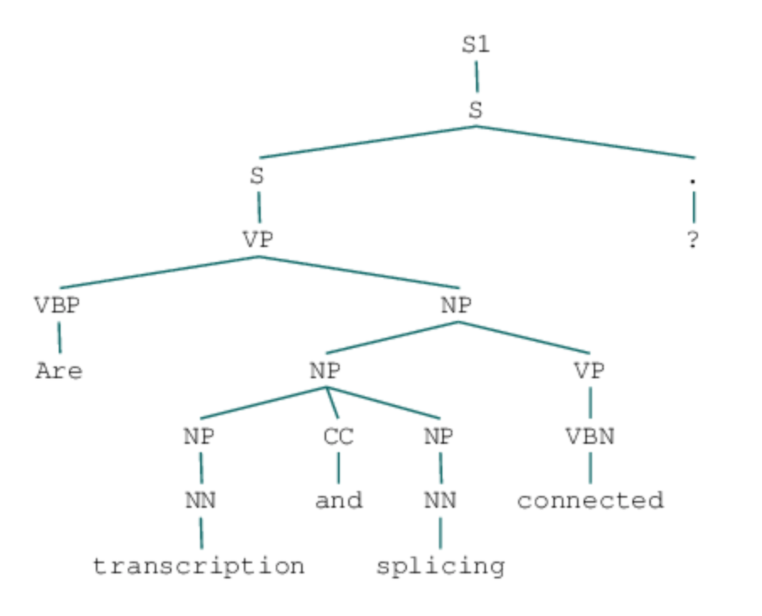
\includegraphics[scale=0.5]{images/question_parse.png}
    \caption{The parse tree of an example question as generated by the BLLIP parser}
    \label{fig:parse_tree}
\end{figure}

\subsubsection{Assertion Extraction}

The first step towards answering the question is to identity the assertions made by the question. To extract the assertions from the question, we use a statistical natural language parser to identify the syntactical structure in the question. We, then, heuristically generate assertions from the questions.\\
Consider the following example question: \\

\textit{Is the monoclonal antibody Trastuzumab (Herceptin) of potential use in the treatment of prostate cancer?} \\

Upon parsing of this question, we have the phase constituents of the question. As shown in the example in \label{fig:parse_tree}, almost all yes/no questions have a standard format that begins with an auxilary verb followed by a noun phrase. In this example, we can toggle the question word with the first noun phrase to generate the assertion: \\

\textit{The monoclonal antibody Trastuzumab (Herceptin) is of potential use in the treatment of prostate cancer.} \\

In a similar manner, we then create positive assertions for all \textit{yes/no} questions as depicted in Figure . As a simple extension to this, we can also create negative assertions by using \textit{not} along with the auxiliary verbs.

\begin{table*}[t!]
    \centering
    \begin{tabular}{r l} \hline
        Question & Assertion \\ \hline
    \textit{Is} the protein Papilin secreted? & The protein Papilin \textit{is} secreted \\
    \textit{Are} long non coding RNAs spliced? & 
    long non coding RNAs \textit{are} spliced \\
    \textit{Are} transcription and splicing connected? &
    Transcription and splicing \textit{are} connected. \\
    \textit{Is} RANKL secreted from the cells? &
    RANKL \textit{is} secreted from the cells. \\
    \textit{Does} metformin interfere thyroxine absorption? & 
    Metformin \textit{does} interfere thyroxine absorption. \\
    \textit{Has} Denosumab (Prolia) been approved by FDA? &
    Denosumab (Prolia) \textit{has} been approved by FDA. \\
    % \textit{Is} Alu hypomethylation associated with breast cancer? & 
    % Alu hypomethylation \textit{is} associated with breast cancer  \\
    \hline
   \end{tabular}
    \caption{Assertion generation for some questions from training set in BioASQ Phase 6b by heuristic-based rearrangement of the auxiliary verb the questions starts with.}    \label{tab:assertion_examples}
\end{table*}

\subsubsection{Recognizing Textual Entailment}

The primary goal of our system is to infer if any of the sentences among the snippets entails or contradicts the assertion made by the question. With the positive and negative assertions from a question, we segmented the snippets for the question to get a set of assertion-sentence pairs. To then evaluate if these assertions can be inferred or refuted from the sentences, we built a Recognizing textual entailment model. Considering how most state-of-the-art textual entailment models are deep RNN-based neural models, we used one such neural model, \textit{InferSent} \cite{Infersent} , that computes sentence embeddings for every sentence and has been shown to work well on NLI tasks. In training \textit{InferSent}, we experienced two major challenges:

\begin{enumerate}
    \item The number of assertion-sentence pairs in BioASQ is too few to train the textual entailment model effectively
    \item The models that are pre-trained on SNLI \cite{snli}
    datasets use GLOVE \cite{glove} embeddings that cannot be used for biomedical corpora which have quite different characteristics and vocabulary compared to the corpora that GLOVE was trained on
\end{enumerate}

However, we have pre-trained embeddings available that were trained on PubMed and PMC texts along with Wikipedia articles \cite{biomed_embed}. To leverage these embeddings, we implemented an embedding-transformation methodology to projecting the PubMed embeddings to GLOVE embedding space and then fine tune the pre-trained \textit{InferSent} on the BioASQ dataset for textual entailment. The hypothesis is that, since both the embeddings had a significant fraction of documents in common (Wikipedia corpus), by transforming the embeddings from one space to another, the sentence embeddings from the model would still represent a lot of the semantic features of the input sentences that can subsequently used for classifying textual entailment. For this task, we explored two types of transformations:

\begin{enumerate}
    \item \textbf{Linear transformation}
    While simple, a linear projection of embeddings from one space to another have shown to be quite effective for a lot of multi-domain tasks. By imposing an orthogonality constraint on the project matrix, we model this problem as an orthogonal Procrustes problem: \\
    Let $d_p$ and $d_g$ be the embedding dimensions of PubMed embeddings and GLOVE embeddings respectively.
    If $E_p$ and $E_g$ are the matrices of PubMed embeddings ($N \times d_p$) and their corresponding GLOVE embeddings ($N \times d_g$) for the words that both the embeddings have in common ($N$), the projection matrix ($d_g \times d_p$) can be computed as,
    \begin{align*}
        W^* &= \argmin_W \lVert  W E_p^{\intercal} - E_g^{\intercal} \rVert
    \end{align*}
    subject to the constraint that $W$ is orthogonal.
    The solution to this optimization problem is given by using the singular value decomposition of $E_g^{\intercal} E_p$, i.e.
    \begin{align*}
        W^* &= UV^{\intercal}, \\
        \text{where, } \\
        E_g^{\intercal} E_p &= U \Sigma V^{\intercal}
    \end{align*}
    With this simple linear transformation, we then computed the transformed embeddings for all the words in the PubMed embeddings that are not present in the GLOVE embeddings. 
    \item \textbf{Non-linear transformation}
    For non-linear transformation, the objective is to learn function $f$ such that,
    \begin{align*}
        f(e_p; \theta) = e_g
    \end{align*}
    where, $e_p$ and $e_g$ are PubMed and GLOVE embeddings respectively. We model $f$ using a deep neural network with parameters $\theta$, and train using the common words in both the embeddings. The effectiveness of this training is a result of the large number of common vocabulary between the two embeddings (since both are trained on Wikipedia text among other corpora).

    \end{enumerate}

    The transformed embeddings from these models were used in conjunction with the pre-trained \textit{InferSent} model to encode the semantic features of the biomedical sentences as sentence embeddings. Subsequently, we employ these sentence embeddings of the assertion-sentence pairs for a particular question to train a three-way neural classifier to predict if the relationship between the two is entailment, contradiction or neither. 
    
    It is worth noting here that the embedding transformation techniques that we implemented are not specific to the NLI tasks and, in fact, enable transfer learning of a much broader set of tasks on smaller datasets like BioASQ by using the pre-trained models on large datasets of other domains and fine-tuning on the smaller dataset.
    

    \subsubsection{Classification}
    
    As a final step, we use the textual entailment results for each assertion-sentence pair generated to heuristically classify the answer as \textit{yes} or \textit{no}. Since our system comprises multiple stages with the errors of each cascading to the final stage, we do not get perfect entailment results for the pairs. However, since we have a lot of pairs, we aggregate these entailment scores to compute the overall entailment or contraction scores to reduce the effect of accumulated errors for individual pairs on classification.
    
    We used a simple unsupervised approach for classification by just comparing the overall entailment and contradiction scores, i.e. if the total number of snippet sentences that entail the assertion are $N_e$ and the total number of snippet sentences that contradict are $N_c$, then, 
    
    \begin{align*}
        \text{answer}_{\text{q}} = \begin{cases}
        \text{yes} & \text{if } N_e \ge N_c \\
        \text{no} & \text{ otherwise}
        \end{cases}
    \end{align*}

    \begin{figure*}[t!]
        \centering
        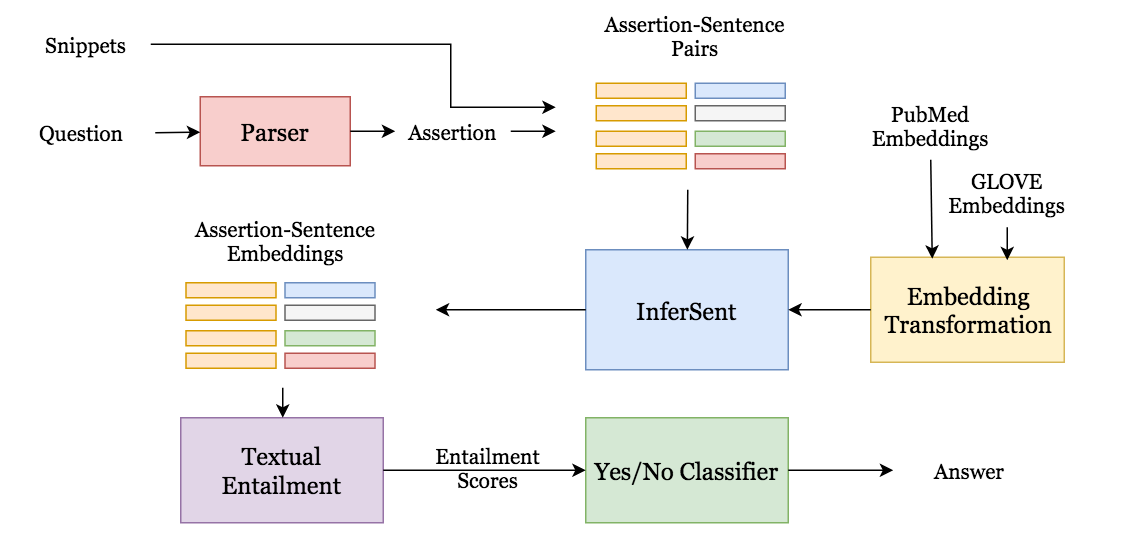
\includegraphics[scale=0.3]{images/YesNoPipeline.png}
        \caption{The complete system for yes/no answer classification using a question and relevant snippets}
        \label{fig:yesno_pipeline}
    \end{figure*}

    The end-to-end architecture of our system from the input questions and snippets to the answer is shown Figure \ref{fig:yesno_pipeline}.
    
\subsubsection{Experimental Details}

For parsing the questions, we used BLLIP reranking parser \cite{charniak_new1} (Charniak-Johnson parser) %\cite{charniak_new1} 
and used the model \texttt{GENIA+PubMed} for biomedical text. For training the textual entailment classifier using \textit{InferSent}'s sentence embeddings, we used Stanford's SNLI \& Multi-NLI dataset \cite{snli} to achieve a test-set accuracy of $84.7 \%$.
%TODO: Specify details for non-linear embedding transformation

\subsubsection{Results}

The performance of the system on yes/no questions on the training set of phase 6b has been tabulated in table \ref{tab:yesno_results}. We notice that, while the accuracies are better than a random classifier, the task is far from being solved. However, the classifier does handle the class bias in the training data and performance similarly on both the categories of answers. While we implemented a simple heuristic based answer-classifier, we believe that a supervised classifier using the sentence embeddings as well as fine-tuning of the textual entailment classifier on BioASQ dataset would considerably enhance the overall performance of the system.

\begin{table}[t!]
    \centering
    \begin{tabular}{c|l} \hline
    
    Category & Accuracy (\%) \\ \hline
    Yes      &  58.4  (306/524)\\
    No       &  63.0 (58/92) \\
    Overall  &  59.1 (364/616) \\      \hline
    \end{tabular}
    \caption{Class-wise accuracies on yes/no questions in training set of BioASQ Phase 6b}
    \label{tab:yesno_results}
\end{table}

\subsection{Factoid \& List Type Questions}

The key objective in extraction-based factoid and list type question answering systems is to find a subset of entities (or phrases) from the relevant snippets that are most likely to answer the question. Most state-of-the-art models for this task involve training end-to-end deep neural architectures to identify these entities. But, owing to the small size of the dataset, we cannot effectively train such models on the BioASQ dataset. Hence, we adopted a two-stage approach that first uses an ensemble of Named Entity Taggers to identify the entities that could potentially answer the question and a supervised classifier to rank the entities on the basis of their likelihood of answering the question.

For devising the model and evaluation, we primarily focused on factoid type questions since the methodology for the list-type question would be largely similar and different only in the number of top entities returned. 

\begin{table}[h]
    \centering
    \begin{tabular}{cccc} \hline
    \multirow{3}{*}{NER Tags} & 
    \multicolumn{2}{c}{\% of questions} & 
     \% of \\
    & Exactly & Partially & tokens \\
    & Answered & Answered & extracted \\ \hline
    PubTator & 32.05 &	72.15 & 52.27 \\
    Gram CNN & 34.90 &	99.03 & 94.97 \\
    LingPipe & 26.67 &	76.75 & 11.06 \\
    Union    & 49.04 &	99.65 & 99.25 \\
    Intersection & 16.29 &	38.00 & 3.33 \\ \hline
    \end{tabular}
    \caption{Baseline recall performances of different NER Taggers evaluated by the fraction of questions that can be answered by an ideal classifier if the candidates are chosen using the tagger. We also indicate a precision measure by evaluating the fraction of total unique tokens form the documents that are tagged.}
    \label{tab:NER_tagging_performances}
\end{table}

\begin{table*}[t!]
    \centering
    \begin{tabular}{|c|c|c|c|c|} 
    \hline \hline
    Model & Exact Answers & Exact Answers & Exact Answers & Ideal Answers \\
    &Yes/No type& Factoid  type& List type & All types \\
    & Accuracy (\%) & MRR & F1 score & ROUGE-2\\
    \hline \hline
    \cite{khyati-paper} & - & - & - & 0.653  \\
    \hline
    \cite{fudan}&\textbf{0.714}&0.272& 0.187& -\\
    \hline
    \cite{fastqa}& - &0.392& 0.361&-\\
    \hline
    Sarrouti and Alaoui \shortcite{usmba}&0.461&0.207&0.243&0.577\\
    \hline
    \textit{BioAMA}(Ours)&0.591&&&\textbf{0.721}\\
    \hline \hline
    
    \end{tabular}
    \caption{Comparison of our model with other state of the art approaches}
    \label{tab:comparison_results}
\end{table*}

\subsubsection{Candidate Selection}

We found that the most critical step in the answer generation process is to identify the set of potential answer candidates that can be fed into a classifier or ranker to identify the best candidates. To accomplish this, we used Named Entity Recognition (NER) taggers to form a set of candidate answers, since almost all the factoid and list answers are named entities. The taggers that we used include Gram-CNN \cite{gram-cnn}, LingPipe\cite{lingpipe} and PubTator \cite{pubtator}. In order to analyze the effectiveness of each of these NER taggers as well as their union and intersection, we perform an analysis on BioASQ training set 5b by evaluating the fraction of questions whose answers are included in the candidate entity set by the taggers.

Table \ref{tab:NER_tagging_performances} shows the relative performances of the three taggers, their union as well as intersection on train dataset of BioASQ 5b factoid type questions. A question is exactly answered if a tagger tags an entity that matches an answer exactly, and it is partially answered if there is a non-zero overlap with an entity tagged and an answer for the question. We can notice that PubTator and LingPipe have a good recall with relatively low precision, while Gram CNN has high recall but low precision.


\subsubsection{Classification Features}\label{sec:classification_features}

Upon computing the set of candidate answers, we use the question $q$, set of relevant snippet sentences $\mathcal{S}$ and entity type $t_i$ to devise a feature vector for each individual entity $e_i$ that comprises the following features:

\begin{enumerate}
    \item[i] BM25 Score: The BM25 scores for all the sentences are computed with the question as the query. Then, the scores of the sentence that contain the entity are aggregated to compute the BM25 score for the entity, i.e.
    \begin{align*}
        \text{BM25 }&\text{Score($e_i$)} \\
       &= \sum_{s \in \mathcal{S}} \text{BM25 Score($e_i$)} \cdot \mathbbm{1}(s, e_i)
    \end{align*}
    where $\mathbbm{1}(s, e_i)$ is 1 iff sentence $s$ contains entity $e_i$.
    \item[ii] Indri Score: Computed in the same manner as BM25 score in (i)
    \item[iii] Number of Sentences: Number of sentences $s \in \mathcal{S}$ that contain the entity $e_i$
    \item[iv] NER Tagger: A multinomial feature that represents which tagger amongst PubTator, LingPipe and GramCNN the entity was extracted with. This feature is included to identify the relative strengths of the different taggers.
    \item[v] Tf Idf: The aggregate Tf-Idf scores of the entity with $\mathcal{S}$ as the set of documents
    \item[vi] Entity Type: Is a boolean feature that is 1 if the type of the entity (for example, \textit{gene}) is present in the question, and 0 otherwise.

\end{enumerate}

\subsubsection{Unsupervised Ranking}

As a baseline, we first present an unsupervised ranking system for the candidate answers. In this system, the snippet sentences are first ranked using the BM25 model. Then, for each entity, a score is computed by aggregating the BM25 scores of the sentences in which the entity is present. The rationale for this is that the entities in the top ranked sentences are more likely to be the answers. This entity score (which is equivalent to the BM25 score described in \ref{sec:classification_features}) is then used to rank the entities and return the top $k$ entities as answers to the question. The overall unsupervised system is shown in Figure \ref{fig:UnsupervisedNERPipeline}.

\begin{figure}
    \centering
    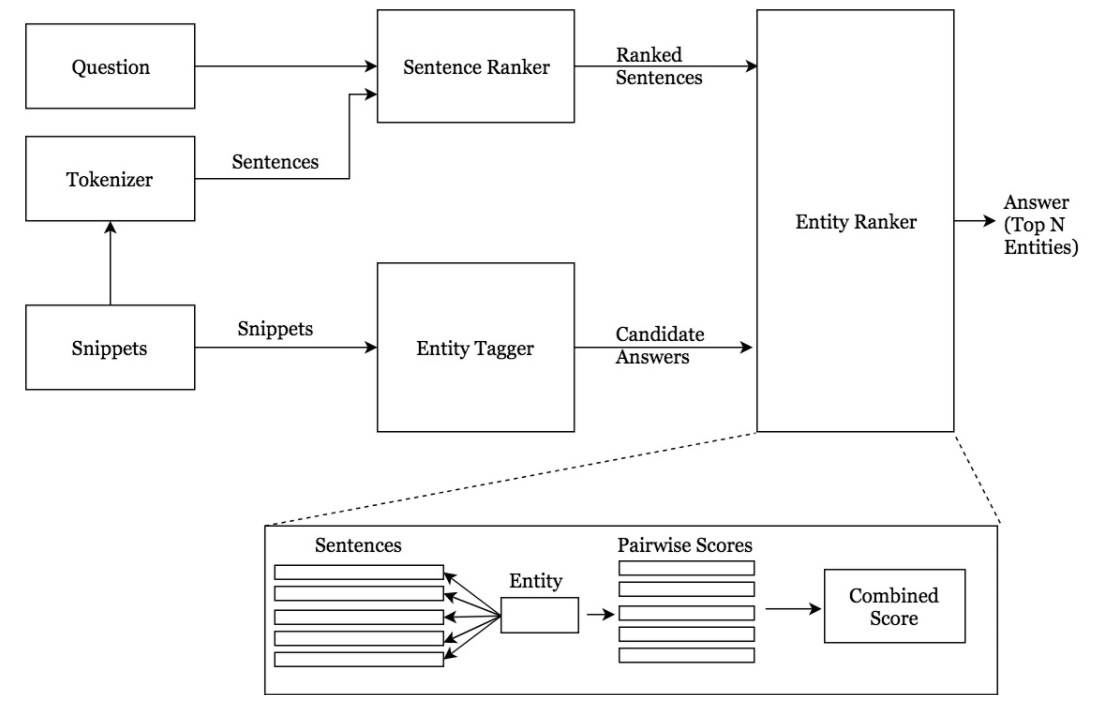
\includegraphics[scale=0.4]{UnsupervisedNERPipeline.png}
    \caption{Unsupervised generation of factoid/list type answers using NER taggers and BM25 retrieval model}
    \label{fig:UnsupervisedNERPipeline}
\end{figure}

\subsubsection{Learning To Rank}

In order to rank the candidate entities in a supervised way, we used a ranking classifier based on the features described in \ref{sec:classification_features}. For ranking, we chose pairwise ranking classifiers over point-wise and list-wise, because they have been known to work better in practice for precision and since we are concerned more about ranking than the actual scores. We are using a traditional SVM-Light \cite{svmlight} implementation for pairwise ranking which is known to give strong results for ranking tasks.

The data for supervision was derived from the actual answers to the question in train data. The candidate entities were ranked based on their overlap with the actual answers, and the model was trained to learn these rankings.

% The idea behind our approach for factoid and list types of questions are based on pairwise Learning To Rank (LeToR). Each questions consists of a group of snippets and the actual query body. Given a Candidates Space (C) of possible named entities, a query (q) and a group of sentences extracted from the snippets (S); our approach is to train a model which ranks each candidate c of C given S and q. Basically, we are learning a function $g(c_i,c_k,S,q)$ that incorporates a score for each pair ($c_i,c_k$) of the Candidates Space. With the respective rankings, we can create a ranked list of entities to be returned. Therefore, in order to execute the model, it's necessary to define a Candidates Space C; a feature vector for each combination $f(c_i,S,q)$; and a function g for $g(c_i,c_k,S,q)$.

Once we rank the entities, we use a naive approach of merely taking top 5 entities as answers for factoid type and top 10 for list-type. One could, however, devise a separate model for identifying the number of top entities to return as answers for the list-type answers.

% \newline \textbf{Features}: For features, we have used combination of syntactic, information retrieval, information theory, semantic and lexical features. POS tags, frequency, tf-idf, NER tags are examples of the features extracted for each candidate representation, which would consist of a vector of values between 0 and 1.  Therefore, for each candidate answer c for a question, we have a vector $v = f(c_i,S,q)$ that represents the features for this candidate.

% By directly testing and combining results, we decided to use the union of PubTator and LingPipe entities to build our Candidate Space. However, this was an insufficient approach due to the fact that it was too narrow to actually achieve reasonable results. Although the features chosen and the ranking model worked well, there was an upper bound precision available by this approach. Therefore, we shifted for different approaches: Noun's combinations, entity recognition systems not related to the biological domain and noun phrases. Noun Phrases have shown the best results: they are a large enough space (it doesn't create a hard bound limit for our results), but still possible to search and rank.

\subsubsection{Results}


\begin{table}[t!]
    \centering
    \begin{tabular}{ccc} \hline
    Entities & Soft Accuracy (\%) & MRR (\%) \\ \hline
    Pubtator & \textbf{7.14} & 3.35 \\
    Lingpipe & 4.58 & 2.70 \\
    Gram CNN & 0.98 & 0.24 \\
    Union    & 1.05 & 0.38 \\
    Intersection & 4.91 & \textbf{3.68} \\ \hline
    \end{tabular}
    \caption{Performance of unsupervised ranking model to identify the entities among the candidates from different taggers, for factoid type questions in BioASQ 5b dataset}
    \label{tab:my_label}
\end{table}

% Model	Exact Matches	Soft Matches	MRR Exact
% Pubtator	7.14%	50.71%	3.35%
% Lingpipe	4.58%	60.72%	2.70%
% Gram CNN	0.98%	85.53%	0.24%
% Ensemble Union	1.05%	85.29%	0.38%
% Ensemble Intersection	4.91%	39.47%	3.68%

\section{Conclusion and Future Work}
\label{future}
In this paper, we present a framework for tackling both ideal and exact answer type questions and obtain state of the art results on the ideal answer type questions on the BioASQ dataset. In our framework for ideal answers, we aimed at improving the Information Retrieval component of the extractive summarization. Although this improved Rogue scores considerably, the human readability aspect of the generated summary answer is not improved to a great extent. We are presently working on using effective abstractive summarization based approaches like Pointer Generator Networks \cite{PGC} and Reinforcement Learning based abstractive summarization techniques \cite{salesforce} to try and improve the human readability aspect of our ideal answers. We aim to continue our research in this direction to adapt these networks to get a good balance between Rogue score and human readability.



% include your own bib file like this:
%\bibliographystyle{acl}
%\bibliography{acl2018}
\bibliography{acl2018}
\bibliographystyle{acl_natbib}

\appendix

\end{document}

\section{Supplemental Material}
\label{sec:supplemental}
ACL 2018 also encourages the submission of supplementary material
to report preprocessing decisions, model parameters, and other details
necessary for the replication of the experiments reported in the 
paper. Seemingly small preprocessing decisions can sometimes make
a large difference in performance, so it is crucial to record such
decisions to precisely characterize state-of-the-art methods.

Nonetheless, supplementary material should be supplementary (rather
than central) to the paper. \textbf{Submissions that misuse the supplementary 
material may be rejected without review.}
Essentially, supplementary material may include explanations or details
of proofs or derivations that do not fit into the paper, lists of
features or feature templates, sample inputs and outputs for a system,
pseudo-code or source code, and data. (Source code and data should
be separate uploads, rather than part of the paper).

The paper should not rely on the supplementary material: while the paper
may refer to and cite the supplementary material and the supplementary material will be available to the
reviewers, they will not be asked to review the
supplementary material.

Appendices ({\em i.e.} supplementary material in the form of proofs, tables,
or pseudo-code) should come after the references, as shown here. Use
\verb|\appendix| before any appendix section to switch the section
numbering over to letters.

\section{Multiple Appendices}
\dots can be gotten by using more than one section. We hope you won't
need that.